O cronograma preliminar das atividades foi baseado de acordo com os prazos para entrega dos relatórios parciais em cada ponto de controle. Como pode ser visto na Figura \ref{fig:cronograma}, o inicio das atividades se deram a partir da escolha do gerente no dia 30/03/2015, e o termino está previsto para o dia 24/06/2015, quando será apresentado o relatório final.
Com o cronograma estabelecido, pode ser elaborado o gráfico de Gantt Figura \ref{fig:gantt}, no qual podemos observar o tempo de execução de cada atividade desenvolvida nas várias etapas do projeto. 

\vfill
 \begin{figure}[H]
	\centering
		\includegraphics[keepaspectratio=true,scale=0.9]{figuras/cronograma.eps}
	\caption{Cronograma de Atividades}
	\label{fig:cronograma}
\end{figure}


 \begin{figure}[H]
	\centering
		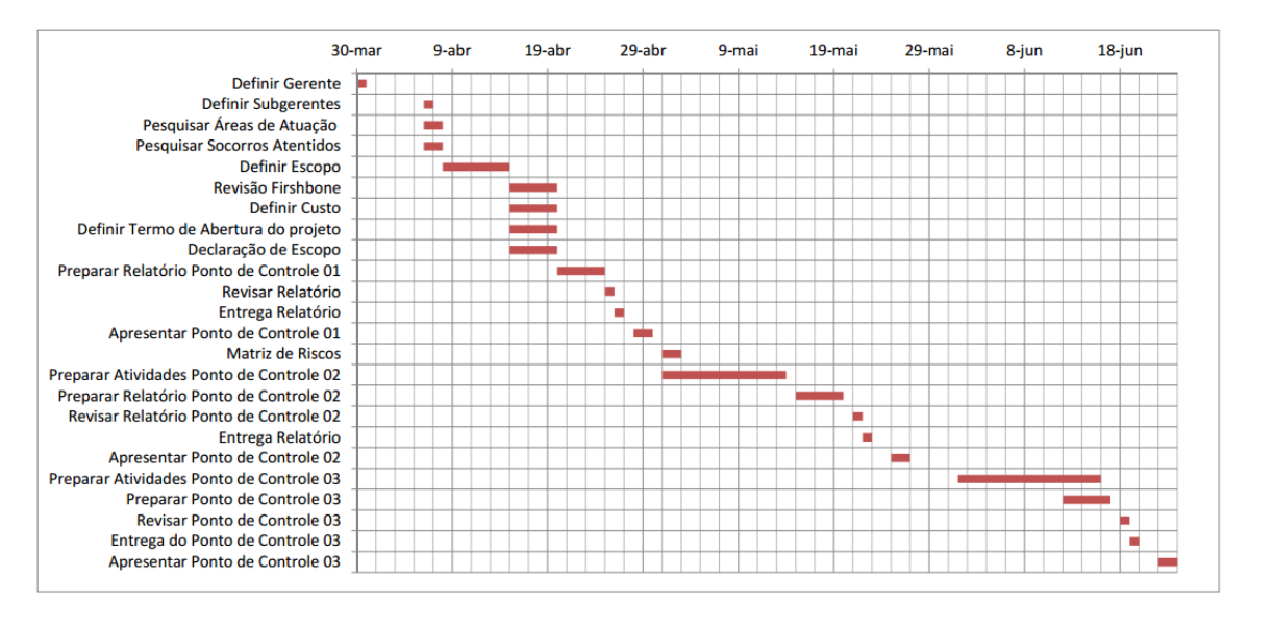
\includegraphics[height=15cm,width=18cm]{figuras/gantt.eps}
	\caption{Gráfico de Gantt}
	\label{fig:gantt}
\end{figure}
